\subsection{Rappresentazione delle Associazioni}

\paragraph{\textcolor{purple}{Uno a Molti}}
Le associazioni \emph{uno a molti} si rappresentano aggiungendo, agli attributi
della relazione rispetto alla quale l'associazione è univoca, una
\emph{chiave esterna} che si riferisce all'altra relazione. Nel caso in
cui l'associazione ha degli attributi si aggiungono anch'essi alla relazione.

\begin{figure}[H]
    \centering
    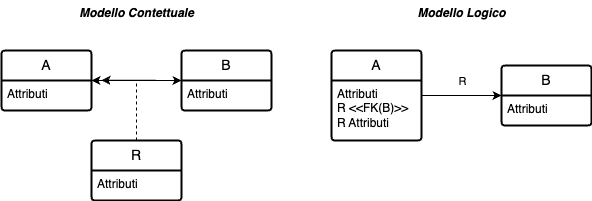
\includegraphics[scale=0.55]{img/unomolti.png}
\end{figure}

\paragraph{\textcolor{purple}{Uno a Uno}}
In questo caso si aggiunge la \emph{chiave esterna}
scegliendo arbitrariamente una delle due relazioni ma, in caso in
cui esiste un vincolo di totalità, si preferisce la relazione
rispetto alla quale l'associazione è \emph{totale}.

\begin{figure}[H]
    \centering
    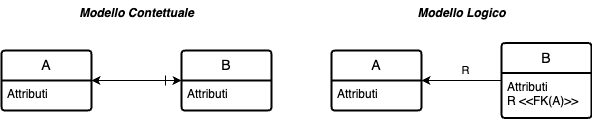
\includegraphics[scale=0.55]{img/unouno.png}
\end{figure}

\paragraph{\textcolor{purple}{Vincoli sulle Cardinalità}} La direzione dell'associazione
rappresentata dalla \emph{chiave esterna} è chiamata la \emph{\textcolor{purple}{diretta}}
dell'associazione. Per imporre un vincolo di \textcolor{purple}{univocità} della diretta occorre definire
un vincolo di chiave sulla \emph{chiave esterna}; mentre per descrivere un vincolo di \textcolor{purple}{totalità}
della diretta si impone un vincolo \verb|NOT NULL| sempre sulla \emph{chiave esterna}.

\paragraph{\textcolor{purple}{Molti a Molti}}
Un'associazione \emph{molti a molti} si traduce aggiungendo tra
le due relazioni, una terza che ha come attributi (e come \emph{chiave primaria})
le \emph{chiavi primarie} delle due relazioni.

\begin{figure}[H]
    \centering
    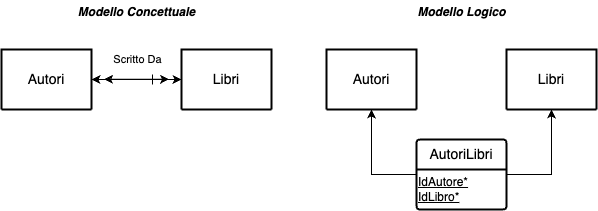
\includegraphics[scale=0.55]{img/moltimolti.png}
\end{figure}

\paragraph{\textcolor{purple}{Ricorsione}}
In questo caso la \emph{chiave esterna} si aggiunge alla stessa e sola
relazione.

\begin{figure}[H]
    \centering
    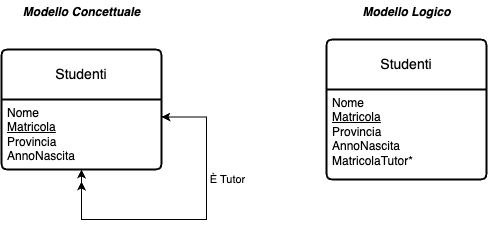
\includegraphics[scale=0.55]{img/ricorsioneunomolti.png}
\end{figure}

\paragraph{\textcolor{purple}{Ricorsione Molti a Molti}}
Anche qui si costruisce una seconda relazione che ha come \emph{chiave primaria}
le due \emph{chiavi primarie} delle due istanze coinvolte.

\begin{figure}[H]
    \centering
    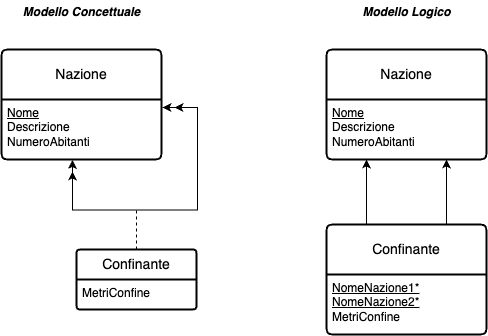
\includegraphics[scale=0.55]{img/ricorsionemoltimolti.png}
\end{figure}

\subsection{Rappresentazione delle Gerarchie}
Le \emph{gerarchie} non possono essere rappresentate direttamente, quindi
vanno eliminate sostituendole con altre classi e relazioni.

Ci sono tre metodi:
\begin{itemize}
    \item \textbf{\textcolor{purple}{Relazione Unica}}: se $A_0$ è la classe genitore di $A_1$ e $A_2$, queste vengono
        eliminate e accorpate ad $A_0$. Ad $A_0$ viene aggiunto un attributo chiamato \textcolor{purple}{discriminatore},
        che indica per ogni istanza da quale classe figlia deriva. Ovviamente anche gli attributi delle classi figlie
        vengono assorbite dal genitore e assumono valore \verb|NULL| sulle istanze di una classe figlia che non possedeva quegli
        attributi. Per quanto riguarda le relazioni, invece, anche queste vengono assorbite dalla classe genitore ma avranno
        comunque cardinalità minima uguale a 0, anche qui per le istanze di una classe figlia che non aveva quella relazione.
    \item \textbf{\textcolor{purple}{Partizionamento Orizzontale}}: la classe genitore $A_0$ viene eliminata e le classi figlie $A_1$
        e $A_2$ ereditano gli attributi e le relazioni del genitore. L'unico caso in cui non si può adoperare questo metodo è quando
        è presente un \emph{vincolo referenziale} verso la classe genitore, in quanto non è possibile spezzare il vincolo
        in più relazioni diverse.
    \item \textbf{\textcolor{purple}{Partizionamento Verticale}}: la gerarchia si trasforma in tante associazioni \emph{uno a uno}
        che legano ogni classe figlia con la classe genitore. In questo caso vanno aggiunti dei vincoli, ovvero ogni istanza di
        $A_0$ non può partecipare a tutte le associazioni, ma ad al più una; e nel caso in cui la gerarchia
        è totale deve essere esattamente 1.
        \paragraph{\textcolor{purple}{Nota Bene}} In quest'ultimo metodo la \emph{chiave primaria} della classe genitore
        è sia \emph{chiave esterna} che \emph{chiave primaria} per le figlie.
\end{itemize}

\subsection{Rappresentazione Campi Multivalore}
Per la gestione dei \emph{\textcolor{purple}{campi multivalore}} viene creata una nuova relazione
che ha come attributi il nome del campo e una \emph{chiave esterna} che si riferisce alla relazione in cui si
trovava. La \emph{chiave primaria} di questa nuova relazione è l'intera ennupla.